\newpage
\section{Gestione domande}
Selezionata la voce \textit{GESTIONE DELLE DOMANDE} dal menù a sinistra il sistema visualizza la seguente pagina, dalla quale un utente può gestire le proprie domande:

\label{GestioneDomande}
\begin{figure}[ht]
	\centering
	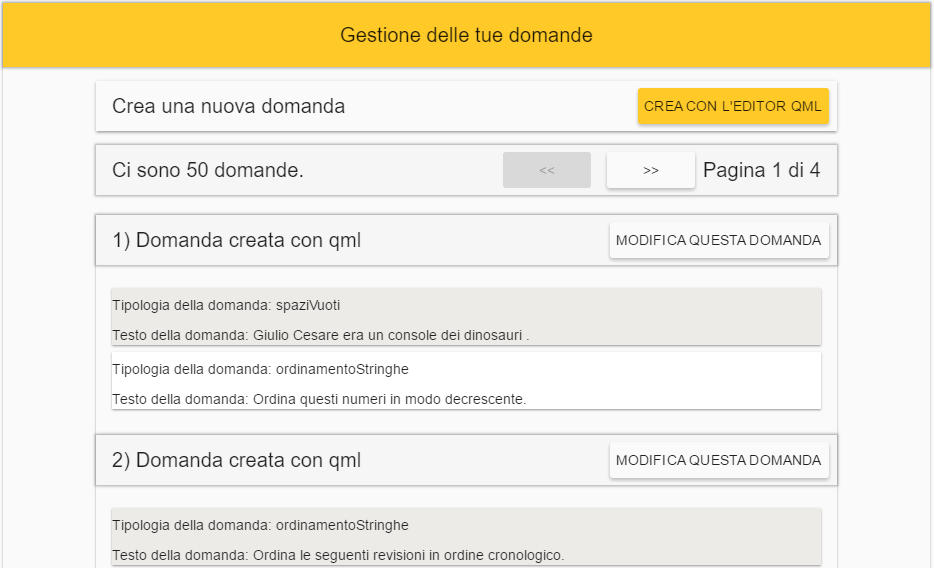
\includegraphics[scale=0.45]{img/gestione_domande.png}
	\caption{Gestione delle domande}
\end{figure}
\FloatBarrier

All'interno della pagina è visibile l'elenco di tutte le domande create, con la possibilità di modificarle. E' possibile poi creare una nuova domanda cliccando sul pulsante \textit{CREA CON L'EDITOR QML}.

\newpage
\subsection{Creazione domanda}
Selezionata la voce \textit{CREA CON L'EDITOR QML} il sistema porta l'utente alla seguente pagina, nella quale potrà creare una nuova domanda digitando codice \textit{QML\ped{G}} (si veda Appendice A) direttamente nell'editor di testo presentato:

\label{CreaDomandaQML}
\begin{figure}[ht]
	\centering
	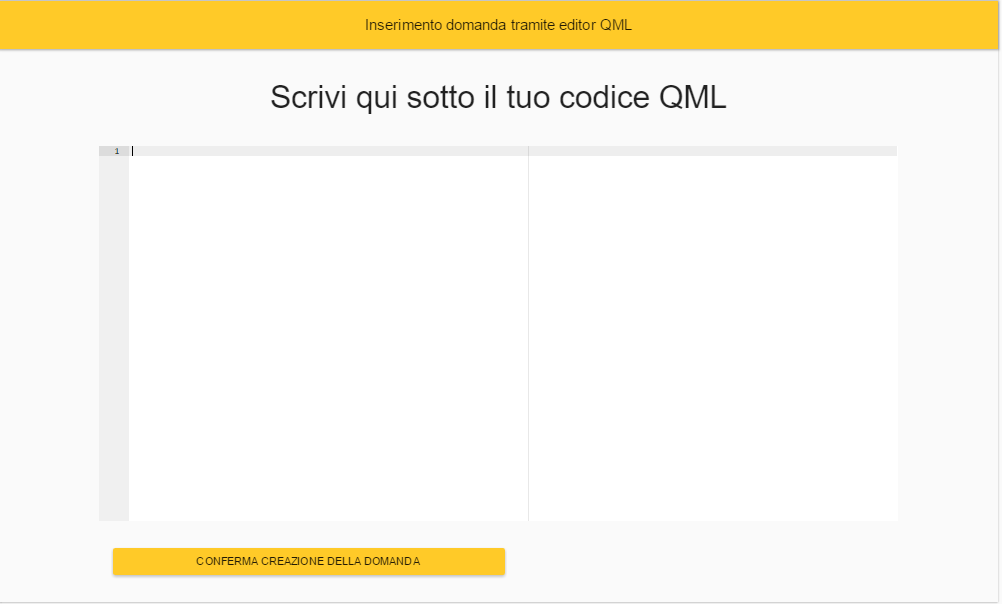
\includegraphics[scale=0.45]{img/creazione_domanda.png}
	\caption{Crea domanda}
\end{figure}
\FloatBarrier

Digitato il corretto codice della domanda nell'editor, sarà possibile cliccare il pulsante \textit{CONFERMA CREAZIONE DELLA DOMANDA} per creare la domanda. Essa sarà così visibile all'interno dell'elenco presentato nella pagina \textit{Gestione domande}.

\newpage
\subsection{Modifica domanda}
Una volta creata, la domanda appare all'interno dell'elenco delle proprie domande. L'utente ha la possibilità di modificarla cliccando sul pulsante \textit{MODIFICA QUESTA DOMANDA} che si trova affianco ad ogni domanda:

\label{ModificaDomanda}
\begin{figure}[ht]
	\centering
	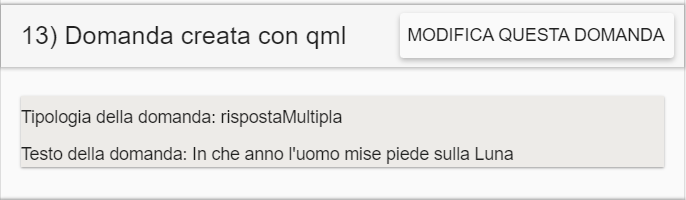
\includegraphics[scale=0.50]{img/modifica_domanda.png}
	\caption{Modifica domanda}
\end{figure}
\FloatBarrier

Viene dunque presentato all'utente l'editor con all'interno la domanda in codice \textit{QML\ped{G}}. L'utente ha la possibilità di modificare il codice ed infine di confermare le modifiche:

\label{ModificaEditor}
\begin{figure}[ht]
	\centering
	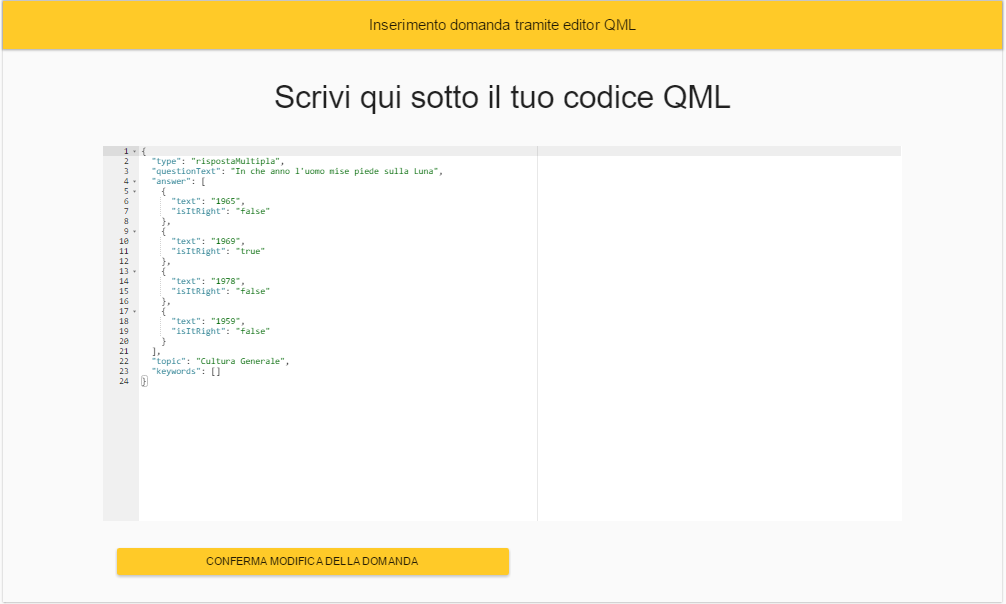
\includegraphics[scale=0.45]{img/modifica_editor.png}
	\caption{Modifica domanda con editor}
\end{figure}
\FloatBarrier 